
Dans ce chapitre, nous présenterons une autre étude de l'interaction entre un utilisateur et un agent virtuel dans le contexte d'une négociation collaborative. 
Notre objectif est d'étudier l'influence de la relation interpersonnelle de dominance sur le processus de négociation. 

En premier lieu, les objectifs généraux de cette étude seront présentés (section \ref{sec:obj}). Nous détaillerons la méthodologie employée pour le paramétrage des agents utilisés dans cette expérimentation (section \ref{sec:methodo}) ainsi que les hypothèses que nous formulons (section \ref{sec:H}).

Nous présenterons ensuite le protocole expérimental employé (section \ref{sec:procedure}). Enfin, nous décrirons les résultats obtenus  (section \ref{sec:res})
que nous discuterons ensuite \ref{sec:discussion}
\section{Objectif}
\label{sec:obj}

Plusieurs études en psychologie sociale ont exploré l'impact de la relation de dominance sur l'expérience de la négociation et de ses résultats. Certains travaux ont montré que l'expression de comportements complémentaires de dominance permettait d'améliorer la coordination et donc le gain commun des négociateurs. En conséquences, les négociateurs se sentaient plus à l'aise. \cite{tiedens2003power,wiltermuth2009benefits,olekalns2013dyadic}.
En parallèle, d'autres travaux ont étudié l'impact de la similarité dans les comportements de dominance dans la négociation. Ces derniers suggèrent que la similarité dans les comportements non verbaux de dominance améliorent l'interaction et le processus de négociation car les individus sont attirés par ceux qui expriment des comportements similaires. Ceci permet d'augmenter le sentiment d'affiliation \cite{olekalns2013dyadic}. 

En vue des contradictions dans la littérature sur l'impact de la complémentarité et la similarité des comportements de dominance dans les interactions, des chercheurs ont mené des études pour comparer les deux approches et étudier laquelle permettait d'avoir de meilleures influences sur l'interaction \cite{tiedens2003power,dryer1997opposites}. Ces études ont montré que la complémentarité de dominance dans les comportements non verbaux s'installait de manière inconsciente entre les individus. De plus, les participants ont préféré interagir avec les individus qui adoptaient un comportement complémentaire et se sentaient plus à l'aise comparés avec ceux qui exhibaient des comportements similaires. 


Partant de ces études, notre objectif est d'explorer l'impact de ces comportements de dominance qu'ils soient complémentaires ou similaires sur les stratégies de négociation dans le contexte d'une négociation collaborative entre un agent et un utilisateur. Cependant, comme la relation de dominance qui s'installe durant l'interaction est forcément complémentaire nous pensons que les stratégies complémentaires auront un impact positif plus important que des stratégies similaires.

\subsection{Complémentarité en psychologie sociale}
	Nous avons présenté dans la section \ref{sec:compEtat} la littérature sur les comportements complémentaires de dominance dans les négociation. Nous rappelons dans cette sections les principaux résultats: 
	
	\begin{itemize}
		\item La complémentarité dans les comportements de dominance améliore la coordination entre les négociateurs qui a pour résultat d'améliore le gain commun des négociateurs.
		
		\item La création de valeurs durant la négociation est plus importante dans des dyades où les négociateurs affichent des comportements complémentaires de dominance
		
		\item En conséquence, le sentiment de confort est accrue dans les dyades complémentaires comparées aux dyades similaires. De plus, la complémentarité permet d'améliorer l'appréciation entre les négociateurs.
	\end{itemize}
	

Nous présentons dans la suite de ce chapitre notre étude qui vise à analyser ces comportements dans le contexte d'une négociation entre un agent et un utilisateur humain.

\section{Méthodologie}
\label{sec:methodo}

Afin d'illustrer notre modèle de négociation, nous reprenons le scénario d'une négociation collaborative pour le choix d'un restaurant.
Ce scénario ne nécessite aucune une expertise pour prendre part dans la négociation. De plus, il est facile pour les participants de reporter leur préférences pour les différents critères pris en compte pour le choix d'un restaurant. En effet, nous considérons le même sujet de négociation des restaurant avec les mêmes critères. Nous avons enrichis le domaine de valeurs des critères. Chaque critère est défini avec un ensemble de valeurs présenté dans la table \ref{tab:valeursCritere}. Un total de 630 restaurants ont été générés à partir des critères regroupant les différentes possibilités.

\begin{table}[b]
	\caption{Ensemble de valeurs possible pour chaque critère afin de choisir un restaurant}
	\label{tab:valeursCritere}
	\centering
	\begin{tabular}{|p{2cm}|p{10cm}|}
		\hline
		\textbf{Critère} & \textbf{Ensemble des valeurs} \\
		\hline
		Cuisine & Chinois ,Français ,Italien ,Japonais ,Coréen ,Mexicain ,Turc \\
		\hline
		Ambiance & cosy ,familial ,anime ,moderne ,romantique ,calme \\
		\hline 
		Prix  & abordable ,bas prix ,chic \\
		\hline
		Localisation & centre de paris ,Gare du nord , Montparnasse , près de la tour Eiffel ,Père lachaise \\
		\hline
	\end{tabular}
\end{table}

Trois paramètres importants sont à prendre en compte pour initialiser les comportements des agents. 
En premier lieu, il faut fixer la valeur initiale de dominance affectée à chaque agent. Nous avons choisi une valeur de dominance $dom =0.55$ afin de générer des comportements de dominance initialement neutres.

En second lieu, il faut initialiser les préférences des agents. Afin de placer les sujets dans des conditions comparables quelles que soient leurs préférences, nous avons demandé aux participants de saisir leur préférences (voir section \ref{sec:procedure}).

A partir des préférences saisies par le participant, nous générons automatiquement les préférences des agents suivant certaines conditions.
La première condition visait à générer des modèles de préférences différents de celui communiqué par l'utilisateur dans le but de créer une confrontation qui pousse à la négociation. Pour cela, nous avons utilisé la distance de kendall \cite{bra2013Kendall}  (\emph{Kendall's  $ \tau \in [0,1]$}) afin de définir la limite minimale de différence entre le modèle de l'agent et celui de l'utilisateur. Par conséquent, nous avons fixer la distance à (\emph{Kendall's  $ \tau \geq 0.7$}).

La seconde condition assurait la différence entre les modèles de préférences générées pour les différents agents qui vont interagir avec les sujets. 
Notre objectif est d'éviter une forte ressemblance entre les préférences des agents qui donnerait l'impression d'interagir avec la même entité.

Nous avons donc gardé uniquement des modèles différents (Kendall's  $ \tau \geq 0.35$). De plus, nous avons ajouté une condition qui assure une différence de perception: pour chaque critère, les modèles devaient avoir des valeurs différentes pour représenter la valeur la plus préférée de l'agent. 
Cela permet de renforcer le sentiment d'interagir avec un agent différent, la valeur préférée étant souvent la première à être proposée par l'agent. 
%Par exemple, considérons deux modèles \emph{P1, P2} générés et qui ont une distance est supérieur à $0.35$. De plus, pour le critère \textit{cuisine}, les deux modèles ont la valeur $Italien$ comme la valeur la plus satisfiable $sat_{P1}(Italien) = 1$ et $sat_{P2}(Italien) = 1$. Ces deux modèles sont automatiquement rejetés.

En dernier lieu, nous avons paramétré la stratégie comportemental des agent. Comme notre but est d'analyser l'impact de la complémentarité ou de la similarité de la dominance durant la négociation, nous avons implémenté trois stratégies distinctes reproduisant les comportements désirés. 
A partir de notre algorithme de la théorie de l'esprit présenté dans le chapitre \ref{chap:Tom}, l'agent calcule la valeur de dominance de l'utilisateur $dom_{user}$ pour chaque tour de parole exprimé par ce dernier. Suivant la valeur de dominance calculée $dom_{user}$, l'agent adopte une des stratégie suivante:


%	Nous avons implémenté trois agents, tous initialisé avec une valeur de dominance
%	De plus, chaque agent adopte une stratégie distincte représentant une condition expérimentale pour notre étude: 

\begin{enumerate}
	\item \textit{Comportement complémentaire}: A chaque tour de parole, l'agent révise sa valeur de dominance pour qu'elle soit complémentaire à celle détécté pour son partenaire $dom_{agent}=1-dom_{user}$.
	
	\item \textit{Comportement similaire}: L'agent va imiter les comportements de dominance exprimés par le participant $dom_{agent} = dom_{user}$.
	
	\item \textit{Comportement neutre} : L'agent ne s'adapte pas à son interlocuteur et suit un comportement de dominance statique.
	
	 $dom_{agent} = dom_{agent} (t=0)$
\end{enumerate}

En modifiant la valeur de dominance de l'agent à chaque tour, nous avons dû ajouter une contrainte dans son modèle décisionnel afin d'assurer une cohérence dans les comportements générés. 
En effet, la valeur de dominance est essentielle pour le calcul des satisfiabilité des valeurs et un changement de cette valeur risque de fausser l'ordre des valeurs satisfiables de l'agent.
Par exemple, à un moment $t$ de la négociation, une valeur $v$ est satisfiable, mais due à une adaptation qui cause un changement de dominance la même valeur $v$ peut devenir non satisfiable. Par conséquent, l'agent peut dire à un tour aimer une valeur et aux tours suivant refuser une proposition pour cette même valeur.

En vue de protéger des préférences et donc la cohérence des comportements de l'agent, nous avons fait le choix d'utiliser uniquement la valeur de dominance initiale $dom_{agent} = 0.55$ pour calculer la satisfiabilité des valeurs.

Nous avons donc implémenté trois agents \emph{Bob, Arthur} et \emph{Kevin}. \emph{Bob} adoptant un comportement complémentaire, \emph{Arthur} qui suit un comportement similaire à celui exprimé par son partenaire de négociation, et enfin \emph{Kevin}, un agent contrôle qui suit une seule stratégie de dominance neutre. 

\section{Hypothèses}
\label{sec:H}

Suivant les travaux de \cite{tiedens2003power,dryer1997opposites,wiltermuth2015benefits}, nous supposons que la relation de dominance établie entre l'agent et l'utilisateur a une influence sur les stratégies exprimées par les négociateurs. Elle va donc avoir une conséquence sur les résultats obtenues lors de la négociation ainsi que le niveau d'appréciation à négocier avec l'agent.
Nous faisons les hypothèses suivantes: 
\begin{itemize}
	\item [$\bullet$] \textbf{H1}: Les comportements de complémentarité et de similarité des agents virtuels sont perçus par les participants.
	\item [$\bullet$] \textbf{H2}: Les négociateurs atteignent un gain commun plus important quand les négociateurs établissent une relation de dominance complémentaire.
	\item [$\bullet$] \textbf{H3}: La négociation converge plus rapidement dans le cas où les négociateurs ont un relation de dominance complémentaire. 
	\item [$\bullet$] \textbf{H4}: Le négociateur se sent plus à l'aise avec un partenaire qui exprime un comportement complémentaire.
	\item [$\bullet$] \textbf{H5}: La complémentarité dans la relation de dominance augmente l'appréciation entre les négociateurs.
\end{itemize}



\section{Protocole expérimentale}
\label{sec:procedure}
Nous présentons dans cette section, le protocole expérimental employé, en commençant par les mesures utilisés pour questionner les participants sur leur interactions. Ensuite, nous présenterons la population de participants et enfin le protocole suivi pour chaque participant. 

\subsection{Mesures}
Après chaque interaction avec un agent, le participant était invité à remplir un questionnaire sur la perception des comportements de dominance.
Nous avons repris les trois principes de dominance (voir section \ref{chap:domer}) pour évaluer les comportements des participants et des agents. De plus, pour chaque questionnaire, nous avons insérés quelques items de manipulation afin de vérifier la concordance des réponses.  Les trois principes représentent quatre comportements de dominance, à savoir :
	\begin{itemize}
		\item \textbf{D1}: La prise en compte des préférences de l'autre dans la prise de décision. Nous avons évalué l'égocentrisme des négociateurs dans leurs stratégies de négociation. 
		\item \textbf{D2}: Le niveau de concessions exprimé durant la négociation.
		\item \textbf{D3}: Le niveau d'exigence du négociateur.
		\item \textbf{D4}: Le négociateur est leader dans la négociation.
	\end{itemize}

\subsubsection{Questionnaire en auto-attribution} Les participants ont répondu pour eux-même au questionnaire des comportements de dominance dans la négociation que nous avons conçu, afin de mesurer les comportements qu'ils ont exhibé durant leur interaction. Ce questionnaire utilise une échelle de Likert à 5 points. Nous présentons ci-dessous les items de ce questionnaire. 
\begin{enumerate}
	\item J'ai été égocentrique pendant la négociation
	\item J'ai pris en compte les préférences de l'agent.
	\item J'ai été exigeant(e).
	\item J'ai maintenu ma position durant la négociation.
	\item J'ai abandonné ma position durant la négociation
	\item J'ai fait des concessions pendant la négociation.	
	\item J'ai mené la négociation.
	\item J'étais leader dans la négociation
\end{enumerate}

\subsubsection{Questionnaire en hétéro-attribution}
Les participants ont répondu à un questionnaire afin de décrire leur perception de l’agent avec lequel ils interagissaient.

Nous nous sommes principalement intéressés aux comportements de dominance exprimés par l'agent. Pour cela, nous avons utilisé le même questionnaire sur les comportements de dominance (voir section \ref{sec:questionnaire})

\subsection{Questionnaire concernant l'interaction}
Pour évaluer l'appréciation du participant vis à vis de l'interaction qu'il a eu avec l'agent. Nous nous sommes basés sur les travaux de \cite{tiedens2003power,wiltermuth2009benefits,olekalns2013dyadic} pour définir le questionnaire ci-dessous:

\begin{enumerate}
	\item Je suis satisfait de la décision finale.
	\item La décision finale était équitable pour nous deux.
	\item Je me suis senti à l'aise pendant la négociation.
	\item J'ai trouvé que la négociation avec l'agent était aisée.
	\item Je me sentais détendu pendant la négociation.
	\item Je me sentais anxieux pendant la négociation.
	\item J'ai apprécié la négociation avec l'agent.
\end{enumerate}

\subsection{Données d'interactions}
Nous avons enregistré les informations suivantes à chaque interaction
\begin{itemize}
	\item Les préférences du participant et celles de l'agent.
	\item Le nombre de tours de négociation avant de trouver un compromis
	\item La position du participant dans le spectre de dominance calculé à partir de l'algorithme de théorie de l'esprit après chaque tour de parole.
	\item Le dialogue généré.
	
\end{itemize}


\subsection{Protocole}
Après avoir expliqué le but de l'étude qui portait sur l'évaluation des comportements d'agents virtuels, l'expérimentateur développait le déroulé de l'étude. 
Premièrement, il expliquait que le but de l'interaction était de négocier avec chaque agent afin de trouver un restaurant où aller dîner. Il leur donnait des instructions afin de se projeter dans une situation réelle en plus de mettre l'accent sur l'aspect "collaboratif" de la négociation comme présenté dans la figure \ref{fig:instruction}.

\begin{figure}[h]
	\fbox{\begin{minipage}{.95\textwidth}
			{\ttfamily
				\textbf{Instruction:} Mettez vous dans la situation où vous allez dîner avec un ami ou un collègue pour la première fois, vous ne connaissez pas ses goûts et il ne connaît pas les vôtres. Le but est de négocier en fonction de vos préférences respectives pour de choisir un restaurant qui \underline{vous convienne à tous les deux}.
			}
		\end{minipage}}
		
		\caption{\label{fig:instruction}Explication du but de l'étude.}
	\end{figure}
	
	
	Une fois le but de l'étude expliqué, l'expérimentateur lançait la phase de tutoriel afin de familiariser le participant à l'utilisation de l'interface de communication. L'expérimentateur présentait les différents les actes de dialogues possibles pour communiquer avec l'agent. 	
	Le participant était informé que durant cette session l'agent ne répondait pas à ses actes, et que le but était uniquement de manipuler l'interface pour générer des actes. 
	
	L’expérimentateur répondait alors à d’éventuelles questions concernant la génération d'actes de dialogue ou leur significations.
	
	Ensuite, l’expérimentateur annonçait au participant qu’il/elle allait négocier avec trois  agents virtuels différents et
	qu’après chaque négociation, il/elle devrait répondre à différents questionnaires pour évaluer son interaction avec l’agent avec lequel il/elle venait de négocier.  Avant de commencer l'expérience, le participant est invité à saisir ses préférences pour les valeurs de chaque critère (voir la figure \ref{fig:pref}).
	
	Une fois les préférences pour les différentes valeurs de critères saisies, la fenêtre avec le premier agent s'ouvrait automatiquement invitant le participant à prendre part à la négociation. 
	
	\begin{figure}[b]
		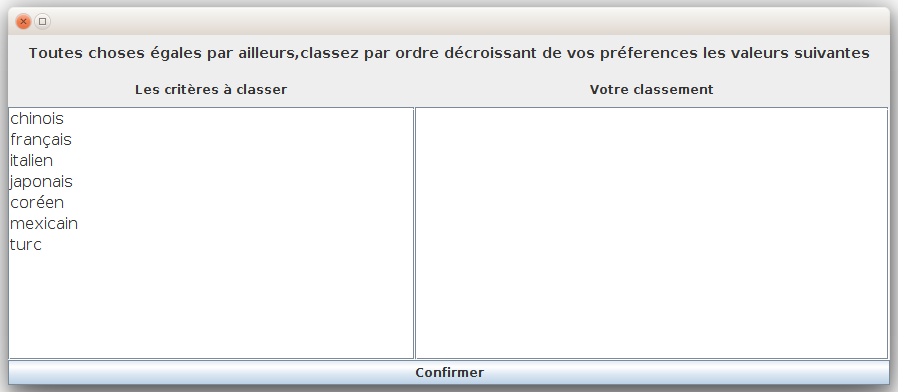
\includegraphics[width=4in]{Figures/pref.png}
		\caption{\label{fig:pref} Interface pour la saisie d'ordre de préférence. Exemple pour le critère de cuisine}
	\end{figure} 
	
	
	\subsection{Hypothèses opérationnelles}
	Nous formulons donc les hypothèses opérationnelles suivantes :
	\begin{itemize}
		\item\textit{\textbf{H1}: Les comportements de complémentarité et de similarité des agents virtuels sont perçus par les participants.}
		
			\subitem $\circ$  Les comportements de dominance attribués par les participants aux agents sont \textit{significativement différents} des comportements de dominance qu'ils se sont auto-attribués.
			\subitem $\circ$ Les comportements de dominance attribués par les participants aux agent sont \textit{similaires} aux comportements de dominance qu'ils se sont auto-attribués.
		
		\item [$\bullet$]\textit{ \textbf{H2}: Les négociateurs atteignent un gain commun plus important quand les négociateurs établissent une relation de dominance complémentaire.}
			\subitem $\circ$ Le restaurant choisi à la fin de la négociation a une valeur de satisfaction  est significativement plus importante pour les préférences des deux négociateurs dans la condition complémentaire comparé aux autres conditions. 
			
		\item [$\bullet$] \textit{\textbf{H3}: La négociation converge plus rapidement dans le cas où les négociateurs ont un relation de dominance complémentaire.}
			\subitem $\circ$ Les participants engageront plus de tours de négociations pour trouver un compromis dans la condition similaire et neutre comparé à la condition complémentaire.
		
		\item [$\bullet$] \textit{\textbf{H4}: Le participant se sent plus à l'aise avec un partenaire qui exprime un comportement complémentaire.}
			\subitem $\circ$ Les scores de \emph{confort} perçus sont plus hauts pour l'agent complémentaire et contrôle que pour l'agent similaire.
			\subitem $\circ$ Les participants trouvent que la négociation est plus aisée avec l'agent complémentaire comparé aux autres agents.
		\item [$\bullet$] \textit{\textbf{H5}: La complémentarité dans la relation de dominance augmente l'appréciation entre les négociateurs.}
			\subitem $\circ$ Les participants vont percevoir l'agent complémentaire comme significativement plus appréciable que l'agent similaire ou neutre.
		
	\end{itemize}
	
	\section{Résultats}
	\label{sec:res}
	Nous avons mené une étude intra-sujet dans laquelle 63 participants ont pris part. Cependant deux participants ont été écarté car ils ne remplissaient pas les conditions requises (mauvaises réponses à la majorité des questions de manipulations). Par conséquent, notre étude statistique a été mené sur les 61 participants restants. 
	
	
	%	Nous avons d'abord analyser la perception des comportements de pouvoir lors de la négociation. En effet, avant d'analyser les hypothèses, nous voudrions étudier la perception des comportements de complémentarité et la similarité durant la négociation. 
	\subsection{Perception des comportements des agents}
	

	\begin{table}[t]
		\caption{Différence de perception de dominance entre l'agent et le participant pour chaque comportement} 
		\centering
		
		\begin{tabular}{ l c c c c c }
			\hline\hline
			\textbf{ }& & \textbf{D1} & \textbf{D2} & \textbf{D3} & \textbf{D4} \\ 
			\hline
			
			\multirow{3}{*} {Agent Comp.}  &  Z-Wilcoxon test  & -4.61 & -5.3 & -6.28 & -0.43 \\ 	
			& p-value & 2.88E-06 & 7.31E-08 & 1.42E-10 & \textbf{0.65 }\\ 
			& Effect size & -0.29 & -0.34 & -0.4 & -0.03\\ 
			\hline
			
			\multirow{3}{*} {Agent similaire}  &  Z-Wilcoxon test  & -1.57 & -2.21 & -1.45 & -1.33\\ 	
			& p-value & 0.11 & \textbf{0.024} & 0.14 & 0.17 \\ 
			& Effect size & -0.1 & -0.14& -0.09 & -0.08 \\ 
			\hline

			\multirow{3}{*} {Agent neutre}  &  Z-Wilcoxon test  & -6.23 & -5.72 & -7.056 & -0.77\\ 	
			& p value & 2.52E-10 & 6.85E-09 & 8.19E-13 & \textbf{0.4351} \\ 
			& Effect size & -0.4 & -0.36 & -0.45 & -0.049 \\ 
			\hline \hline
			
		\end{tabular}
		
		\label{tab:domPercption}
	\end{table}
	
	Pour l'analyse des différences entre les comportements de dominance des agents et des participants, des statistiques non-paramétriques ont été utilisées car la normalité des données ne pouvaient être assurée. Pour l'analyse principale, le test des rangs signés de Wilcoxon a été appliqué pour évaluer chacun des quatre comportements.
	
	\subsubsection{Perception de complémentarité}
	
	Pour chaque comportement, nous avons comparé la perception des participants de leur comportements de dominance et ceux de l'agent complémentaire avec lesquels ils ont interagi. Les statistiques descriptives sont présentées dans la figure \ref{fig:comp}. 
	
	Les résultats de l'analyse de Wilcoxon a révélé que les participants ont perçus une différence significative entre leurs comportements et celui de l'agent comme présenté dans la table \ref{tab:domPercption}. Cette différence concerne les comportements \textbf{D1, D2} et \textbf{D3}. Cependant, aucune différence significative n'a été perçu pour le comportement de leader dans la négociation \textbf{D4}. 
	\begin{figure}[h]
		\centering
		% this is wide enough
		\subfloat [Score de perception des comportements de dominance]{
			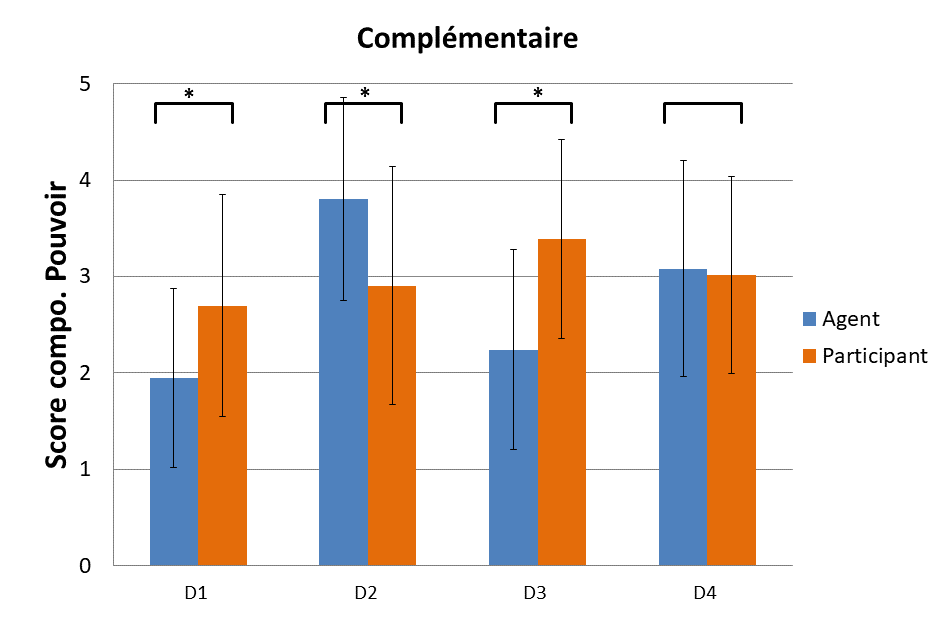
\includegraphics[clip=false]{Figures/chap7/comPow.PNG}
		}
		
		% this has a too narrow subfigure
		\subfloat[Moyenne et écart type dans les comportements de dominance]{
			\begin{tabular}{l c c c c c c}
				\hline\hline
				\multicolumn{2}{c}{} & \textbf{D1} & \textbf{D2} & \textbf{D3} & \textbf{D4} \\
				\hline
				
				\multirow{2}{*}{Agent }& Moyenne & 1,94& 3,80 & 2,24 & 3,08 \\
				& Ecart-type & 0,93 & 1,05 & 1,03 & 1,11 \\
				
				\hline
				\multirow{2}{*}{Participant }& Moyenne & 2,69 & 2,94 & 3,4 & 3,02 \\
				& Ecart-type & 1,14 & 1,23 & 1,03 & 1,02\\
				\hline
				\hline
			\end{tabular}
		}
		\caption{Perception des comportements de dominance avec l'agent complémentaire}
		\label{fig:comp}
	\end{figure}	
	
	\subsubsection{Perception de similarité}
	Nous avons aussi analysé les comportements des négociateurs lors de leurs interactions avec l'agent Arthur. Les statistiques descriptives ont déjà montre une forte similarité dans la perception de tout les comportements (voir la figure \ref{fig:sim}). Nous avons complété l'étude par une comparaison de Wilcoxon a confirmé l'absence de différence significative comme présenté dans la table \ref{tab:domPercption}.  
	\begin{figure}[!tb]
		\centering
		% this is wide enough
		\subfloat[Score de perception des comportements de dominance]{
			\centering
			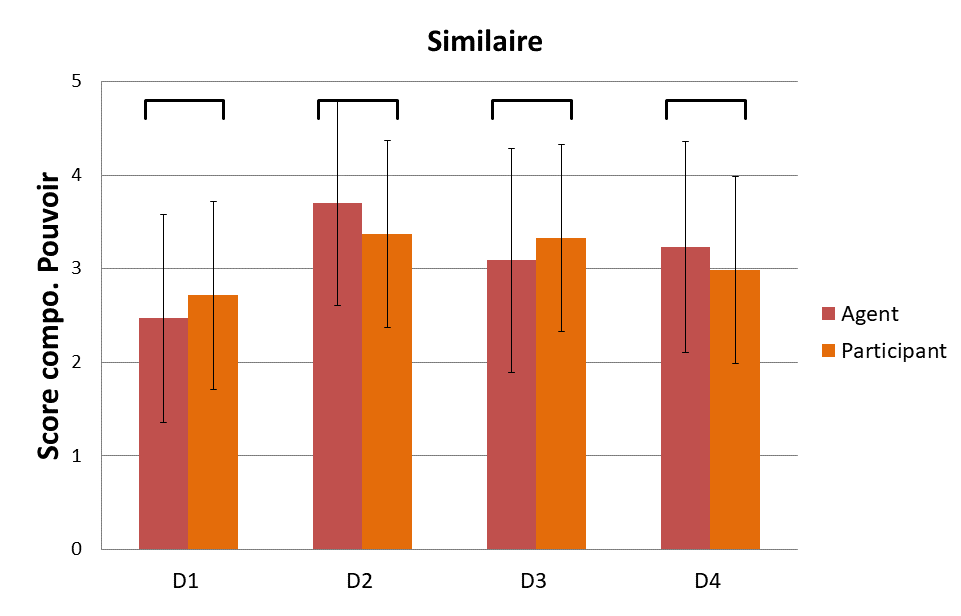
\includegraphics[clip=false]{Figures/chap7/simPow.PNG}
		}
		
		%\vspace{1em}
		% this has a too narrow subfigure
		\subfloat[Moyenne et écart type dans les comportements de dominance]{
			\centering
			\begin{tabular}{l c c c c c c}
				\hline\hline
				\multicolumn{2}{c}{} & \textbf{D1} & \textbf{D2} & \textbf{D3} & \textbf{D4} \\
				\hline
				
				\multirow{2}{*}{Agent }& Moyenne & 2,47 & 3,70 & 3,09 & 3,23 \\
				& Ecart-type & 1,11 & 1,10 & 1,19 & 1,12 \\
				
				\hline
				\multirow{2}{*}{Participant }& Moyenne & 2,71 & 3,37 & 3,33 & 2,98 \\
				& Ecart-type & 1,06 & 1,03 & 1,06 & 1,09\\
				\hline \hline
				
			\end{tabular}
		}
		\caption{Perception des comportements de dominance avec l'agent similaire Arthur}
		\label{fig:sim}
	\end{figure}
	
	\subsubsection{Comportement de l'agent neutre}
	
	Nous avons conduit les mêmes études statistiques pour analyser la perception des comportements de l'agent neutre. L'analyse descriptive présentée dans la figure \ref{fig:neutre} montre que les participants ont perçu que l'agent adoptait une stratégie complémentaire pour les comportements \textbf{D1}, \textbf{D2} et \textbf{D3}. Cependant, aucune différence significative n'a été perçu pour le comportement \textbf{D4}.
	
	\begin{figure}[!tb]
		\centering
		% this is wide enough
		\subfloat[Score de perception des comportements de dominance]{
			
			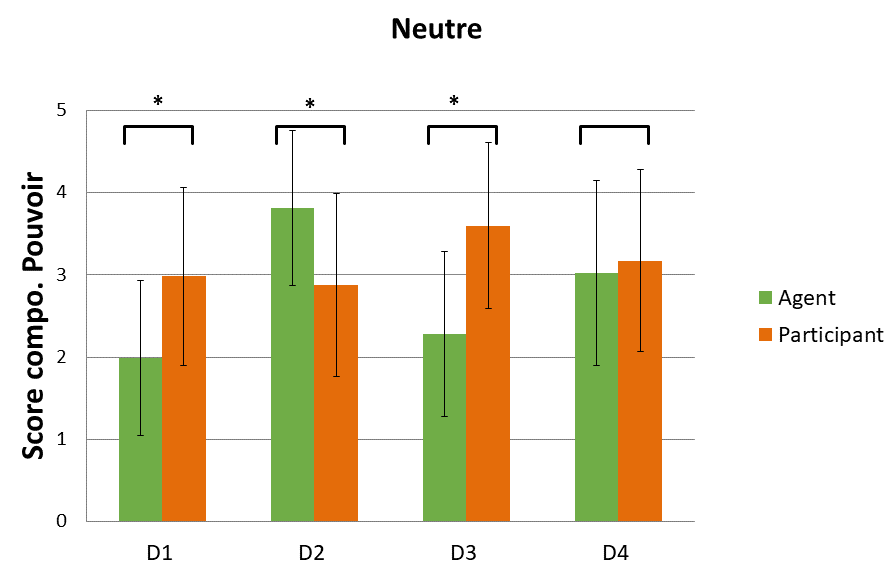
\includegraphics[clip=false]{Figures/chap7/neutrePow.PNG}
		}
		
		%\vspace{1em}
		% this has a too narrow subfigure
		\subfloat[Moyenne et écart type dans les comportements de dominance]{
			
			\begin{tabular}{l c c c c c c}
				\hline\hline
				\multicolumn{2}{c}{} & \textbf{D1} & \textbf{D2} & \textbf{D3} & \textbf{D4} \\
				\hline
				
				\multirow{2}{*}{Agent }& Moyenne & 1,99 & 3,81 & 2,28 & 3,02 \\
				& Ecart-type & 0,94 & 0,94 & 1,01 & 1,12 \\
				
				\hline
				\multirow{2}{*}{Participant }& Moyenne & 2,98 & 2,88 & 3,60 & 3,17 \\
				
				& Ecart-type & 1,08 & 1,12 & 1,01 & 1,10 \\
				\hline \hline
				
			\end{tabular}
			
		}
		\caption{Perception des comportements de dominance avec l'agent neutre}
		\label{fig:neutre}
	\end{figure}
	
	\subsection{Gain commun}
	Nous avons analysé le gain commun des négociateurs durant les différentes négociations. Nous avons d'abord demandé aux participants leurs ressentis sur la satisfaction du restaurant choisi. Nous avons complété cette analyse par une étude objective dans laquelle nous avons calculé le score de satisfaction du restaurant choisi à partir des préférences du participant et de l'agent. L'ensemble des résultats est présenté en Annexe \ref{chap:Annexe}.
	
		\begin{figure}[h]
		
		\centering
		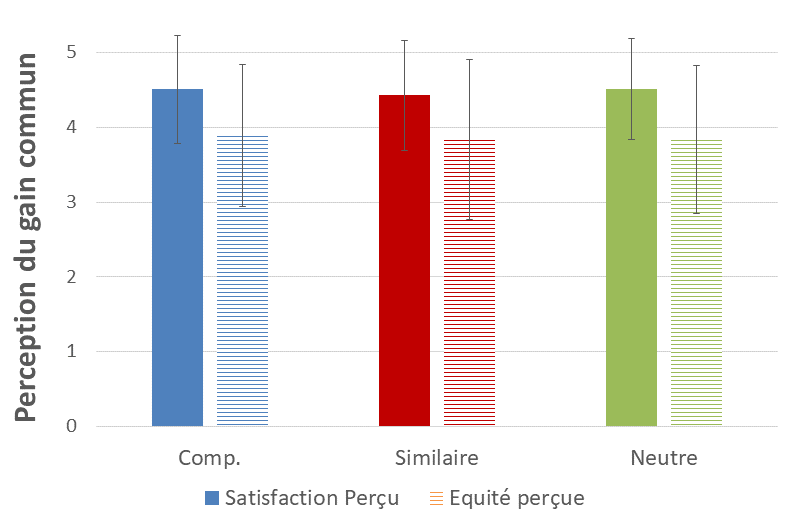
\includegraphics[width= 0.65 \linewidth,clip=false]{Figures/chap7/percpGain.PNG}
		\caption{Perception du gain commun obtenu pour tous les agents \textit{Aucune différence significative entre les agents}}
		\label{fig:gainCom}
	\end{figure}

	\subsubsection{Perception du gain commun} Nous avons demandé aux participants de renseigner leur degrés de satisfaction du restaurant choisi avec l'agent.
	
	Les résultats sont présentés dans la figure \ref{fig:gainCom}. D'abord, les statistiques descriptives montrent qu'en moyenne les participants étaient satisfaits du restaurant choisi, et ce pour toutes les négociations. Les scores sont plutôt supérieurs à la moyenne pour tous les agents (les valeurs varient entre \emph{3.83} et \emph{4.5} sur une échelle de \emph{5}). 
	
	En outre, nous avons analysé si les participants étaient significativement plus satisfaits du restaurants choisi lors de la négociation avec l'agent Bob qu'avec les autres agents. Nous avons effectué un test de rangs signés de Wilcoxon car la normalité des données n'avait pu être assurée. L'analyse n'a montré aucune différence significative de la perception de gain et d'équité sur le choix du restaurant entre les différents agents. 
	
	\subsubsection{Analyse du gain commun } Concernant l'analyse objective du gain commun atteint à la fin de chaque négociation, nous avons dans un premier temps, récupéré les préférences des participants et des agents avec lesquels avaient interagi. 
	Ensuite, nous avons calculé la satisfiabilité du restaurant choisi pour chaque négociateur en fonction de leurs préférences (\textit{i.e l'agent et le participant}). Nous avons ensuite, calculé le gain commun atteint à chaque négociation comme \textbf{la moyenne des valeur de satisfiabilité} des deux négociateurs.  Les résultats obtenus pour chaque agent sont présentés dans la figure \ref{fig:gain}. 
	
		\begin{figure}[h]
		
		\subfloat[Score du gain commun atteint pour tous les agents  \textit{les population regroupées avec $(*)$ sont significativement différentes }]{
			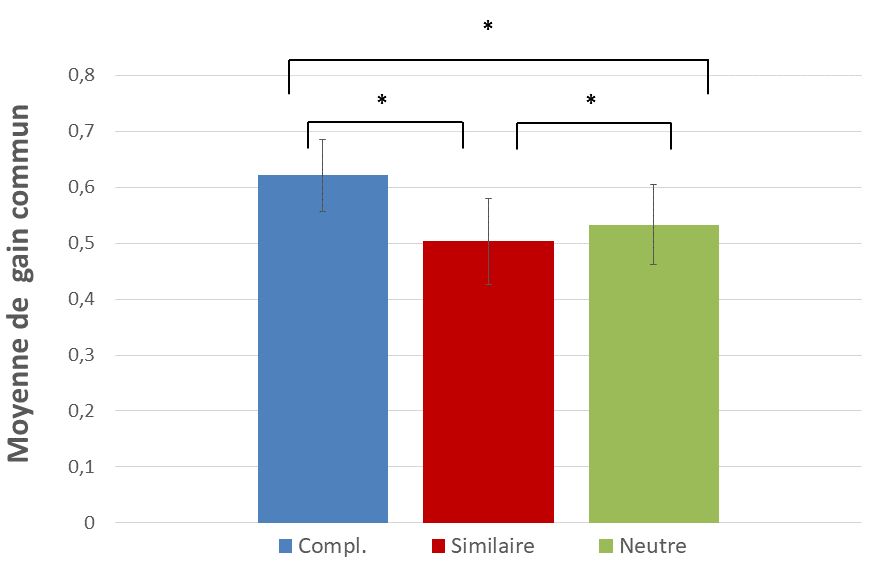
\includegraphics[clip=false]{Figures/chap7/gainCommun.PNG}}
		
		\subfloat [Score du gain commun obtenu par négociation]{
			\centering
			\begin{tabular}{l c c c}
				\hline
				\textbf{ }& \textbf{Agent Comp.} & \textbf{Agent similaire} & \textbf{Agent neutre} \\ 
				\hline
				\newline Moyenne & 0.62& 0.5 & 0.53 \\
				\newline Écart type & 0.06 & 0.08 & 0.07 \\
				\hline
				
			\end{tabular}
		}
		\caption{Les résultats obtenus pour le gain commun atteint durant la négociation}
		\label{fig:gain}
	\end{figure}

	Les valeurs de satisfiabilité sont supérieurs à la moyenne pour tous les agents. Rappelons que les valeurs de satisfiabilité sont normalisées dans un intervalle $[0, 1]$. Nous avons étudié si les négociateurs avaient atteint un gain commun plus importants en négociant avec l'agent complémentaires comparés aux autres agents. En vue de la distributions normales des valeurs, nous avons appliqué un T-test afin de comparer chaque paire d'agents. Les résultats obtenus sont présentés dans la figure \ref{fig:gain}. L'analyse de la variance a montré une interaction significative entre la relation de dominance et le gain commun atteint lors des négociation. Effectivement, les participants ont atteint un gain commun significativement plus élevé en négociant avec l'agent complémentaire qu'avec l'agent similaire (\emph{t= 8.9, p < 0.01}). La même différence a été perçue en comparant avec l'agent neutre (\emph{t= 6.4, p < 0.01}).
	De plus, les participants ont atteint un meilleur gain commun avec l'agent neutre qu'avec l'agent similaire (\emph{t= 2.3, p = 0.02}).
	

	
	\subsection{Tours de paroles}
	
	Pour l'analyse de l'impact de la relation de dominance sur nombres de tours de paroles, nous avons recueilli le nombre de tours de paroles énoncé durant chaque négociation. Les statistiques descriptives sont présentées dans la figure \ref{fig:tour}. Un test paramétrique a été utilisée car les données suivent une distribution normale. Les résultats montrent que la négociation convergeait significative plus rapidement quand les participants négociaient avec l'agent complémentaire par rapport à l'agent similaire (\emph{t= 2.7, p = 0.003}). De même, la négociation convergeait plus rapidement avec l'agent neutre comparé à l'agent similaire (\emph{t= 4.43, p < 0.01}).  Les résultats sont présentés en Annexe \ref{chap:Annexe}.
	Cependant, aucune différence significative n'a été perçu entre l'agent complémentaire et l'agent neutre (\emph{t= 1.3, p = 0.09}).  
	
	\begin{figure}[!tbh]
		
		\subfloat[Nombre de tours de paroles durant une négociation pour tous les agents \textit{les population regroupées avec $(*)$ sont significativement différentes}] {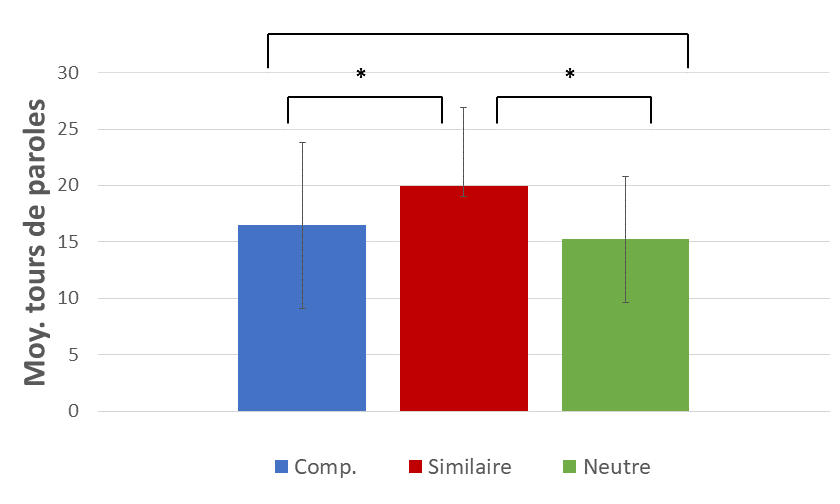
\includegraphics{Figures/chap7/tours.PNG}}
		
		
		\subfloat[Nombre de tours de paroles par négociation]{
			\centering
			\begin{tabular}{ l c c c }
				\hline
				\textbf{ }& \textbf{Agent Comp.} & \textbf{Agent similaire} & \textbf{Agent neutre} \\ 
				\hline
				\newline Moyenne & 16.61& 19.94 & 15.13 \\
				\newline Écart type & 7.38 & 6.87 & 5.6 \\
				\hline
				
			\end{tabular}
		}
		\caption{Résultats pour l'hypothèse H3.}
		\label{fig:tour}
	\end{figure}
	
	
	\subsection{Confort}
	
	Les statistiques descriptives sont présentées dans la table \ref{tab:confort}. Les participants se sont globalement sentis à l'aise avec tous les agents.
	Les score de détente ressentie sont au-dessus de 3,4 (sur une échelle à 5 points) pour tous les agents. Au contraire, les scores relatifs à l'anxiété  ressentie sont au-dessous de 2 (sur une échelle à 5 points) pour tous les agents. 
	
	Afin d'analyser une différence dans le confort perçue, nous avons utilisé un test non paramétrique car la normalité n'a pas pu être assurée. Le test de rang signé de Wilcoxon a été appliqué afin d'analyser si les participants se sont senti plus à l'aise avec l'agent complémentaire qu'avec les autres agents. ( Voir résultats en annexe \ref{chap:Annexe}). 
	Les résultats montrent que les participants se sont senti plus à l'aise avec l'agent complémentaire qu'avec l'agent similaire (\emph{Z= -2.73, p = 0.002})
	avec un effet de taille faible (\emph{e = -0.1}). Cependant, aucune différence significative n'a été perçu entre l'agent complémentaire et l'agent neutre. 
	
	
	\begin{figure}[h]
		
		\subfloat[Score de confort que les participants ont ressenti pour tous les agents. \textit{les population regroupées avec $(*)$ sont significativement différentes }]{
			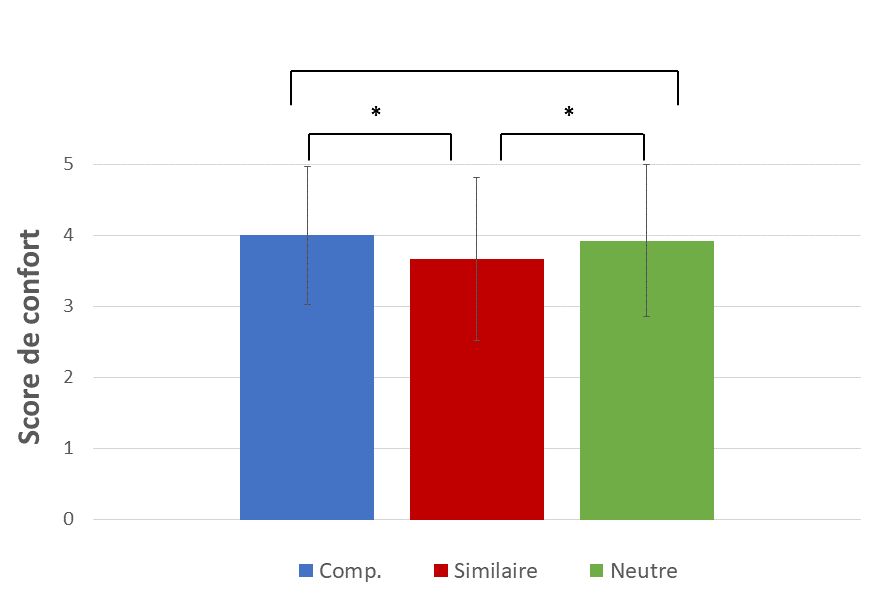
\includegraphics[clip=false]{Figures/chap7/confort.PNG}
		}
		
		\subfloat[L'effet de la relation de dominance sur le confort ressenti pendant la négociation avec l'agent]{
			\centering
			\begin{tabular}{ l l c c c  }
				\hline
				\textbf{ }& & \textbf{Agent Comp.} & \textbf{Agent similaire} & \textbf{Agent neutre} \\ 
				\hline
				\newline \newline\multirow{2}{*} {Détendu} & Moy. &3.79 & 3.47 & 3.79 \\
				\newline  & SD & 1 & 1.2 & 1 \\
				\hline
				
				\newline \newline\multirow{2}{*} {Anxieux} & Moy. & 1.79 & 2.13 & 1.93 \\
				\newline  & SD & 7.38 & 6.87 & 5.6 \\
				\hline
			\end{tabular}
		}
		\caption{Résultats pour la perception du confort durant la négociation.}
		\label{tab:confort}
	\end{figure}	
	\vspace{- 1 em}
	
	\subsection{Appréciation}
	Les statistiques descriptives concernant les scores d’appréciation sont présentées dans la figure \ref{fig:app}. Globalement,
	les scores sont centrés autour de 3.7 (sur une échelle de 5). L'analyse de variance montre l'effet de la relation de dominance sur la perception de l'appréciation. Les résultats sont présentés en annexe \ref{chap:Annexe}.
	
	\begin{figure}[h]
		
		\subfloat[Score d'appréciation perçue pour tous les agents. \textit{les population regroupées avec $(*)$ sont significativement différentes}]{
			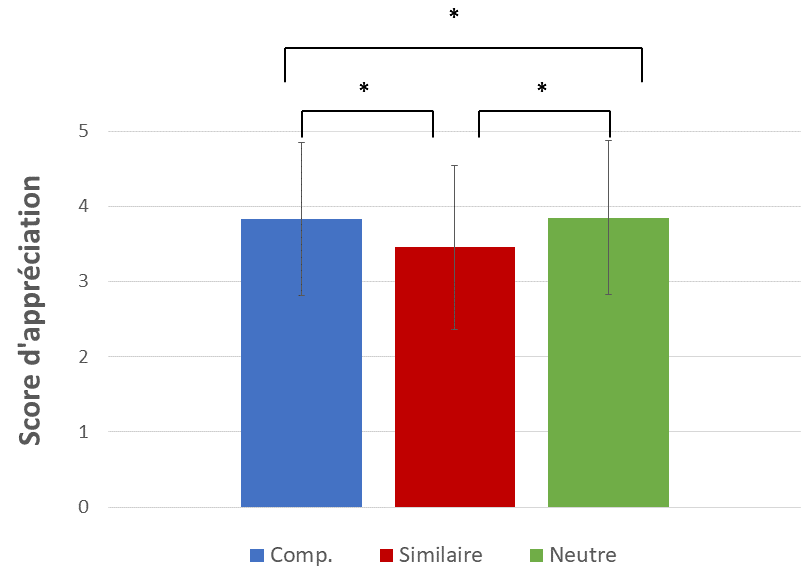
\includegraphics[clip=false]{Figures/chap7/appreciation.PNG}
		}
		
		\subfloat[L'effet de la relation de dominance sur l'appréciation perçue]{			
			
			\begin{tabular}{ l c c c c c }
				\hline
				\textbf{ }& \textbf{Agent Comp.} & &  \textbf{Agent similaire} & & \textbf{Agent neutre} \\ 
				\hline
				\newline Moy. & 3.83 & &3.46 & & 3.85 \\
				\newline SD & 1.01 & & 1.09& &  1.02 \\
				\hline
				
			\end{tabular}
		}
		\caption{Résultats pour la perception de l'appréciation.}
		\label{fig:app}
	\end{figure}
	
	
	Le test de rangs signé de Wilcoxon montre que l'agent complémentaire a été perçu comme significativement plus agréable que l'agent similaire (\emph{p < 0.01, Z = -3.17}). Par ailleurs, l'agent neutre a aussi été perçu comme plus agréable que l'agent similaire (\emph{p < 0.01, Z = -3.3}). Cependant, aucune différence n'a été perçu entre l'agent complémentaire et l'agent neutre (\emph{p = 0.6, Z = -0.31}).
	
	Nous nous sommes aussi intéressé à la facilité de collaboration entre le participant et l'agent. En effet, nous avons demandé aux participants de relater le degrés de facilité de négociation avec l'agent. Les résultats sont présentés dans la figure \ref{fig:aise}. En général, les participants ont trouvé que la négociation été aisée avec l'agent complémentaire (\emph{M= 4, SD = 1}) ainsi qu'avec l'agent neutre (\emph{M=3.9, SD =0.99}). Les participants ont perçue la négociation avec l'agent similaire comme moins aisée (\emph{M=3.16, SD = 1.06 }). 
	Nous avons ensuite analysé si cette différence de perception été significative. Comme les données ne sont pas normalement distribué, nous avons appliqué le test de rangs signé de Wilcoxon. Les résultats montrent qu'en effet les participants ont trouvé que négocier avec l'agent similaire été significativement moins aisée comparé à l'agent complémentaire (\emph{p < 0.01, Z = -3.86} avec un effet de taille moyen \emph{e = -0.35}) et l'agent neutre (\emph{p < 0.01, Z = -3.61} avec un effet de taille moyen \emph{e = -0.32}).
	Cependant, aucune différence n'a été perçue entre l'agent complémentaire et l'agent neutre.
	\begin{figure}[h]
		
		\subfloat[Évaluation de la collaboration durant la négociation. \textit{les population regroupées avec $(*)$ sont significativement différentes }]{
			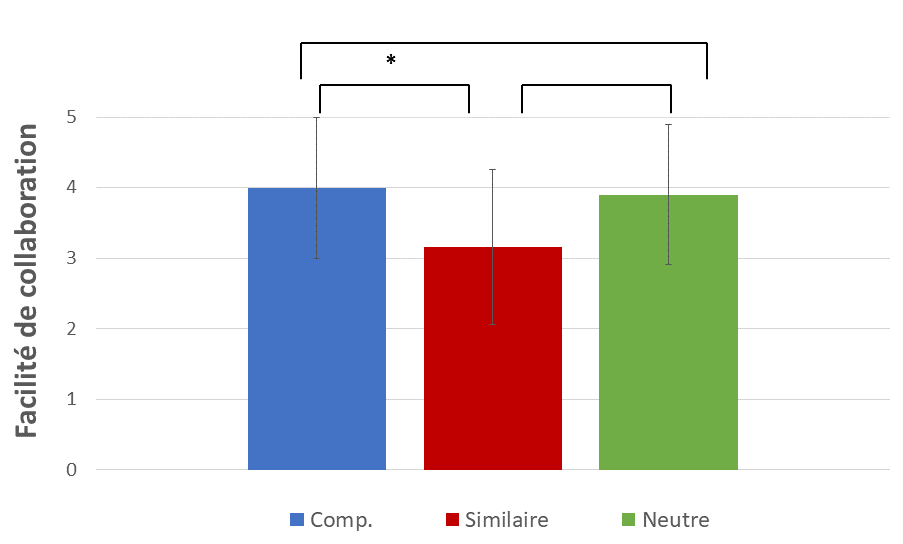
\includegraphics[clip=false]{Figures/chap7/aisee.PNG}
		}
		
		\subfloat[L'effet de la relation de dominance sur la facilité de collaboration]{
			\centering
			\begin{tabular}{ l c c c c c }
				\hline
				\textbf{ }& \textbf{Agent Comp.} & &  \textbf{Agent similaire} & & \textbf{Agent neutre} \\ 
				\hline
				\newline Moy. & 4 & & 3.16 & & 3.9 \\
				\newline SD & 1 & & 1.09  & & 0.99   \\
				\hline
				
			\end{tabular}
		}
		\caption{Résultats pour la facilité de collaboration durant la négociation.}
		\label{fig:aise}
	\end{figure}
	
	
	\section{Analyses complémentaires}
	Dans le chapitre 2, nous présentons la relation de dominance comme une relation interpersonnelle qui s'établie durant l'interaction. 
	Par conséquent, en plus du trais de personnalité, un individu est influencé par l'environnement de l'interaction (\textit{e.g} contexte de l'interaction, rôle social ...). Ces différents paramètres vont créer une certaine relation de dominance qui peut varier d'une interaction à une autre.  
	Afin de vérifier si les participants produisaient différents comportements de dominance durant les différentes négociations, nous avons recueilli la perception de l'agent des comportements de dominance de son interlocuteur.  Les résultats sont présentés dans la figure \ref{fig:dom}.
	
	Nous avons analysé, pour le même participant, la variance des comportements de dominance à travers les trois négociations. Pour ce faire, nous avons utilisé le test de rang signé de Wilcoxon car la normalité des données n'a pu être assurée. 
	
	Les résultats montrent les comportements de dominance des participants variaient d'une interaction à une autre. En effet, le test de Wilcoxon révèle une différence significative entre les comportements perçus par l'agent complémentaire et l'agent similaire (\emph{p<0.01, Z = -3.35}). Ces mêmes résultats sont observé en comparant la perception de l'agent complémentaire et l'agent neutre (\emph{p< 0.01, Z = -3.88}).
	Toutefois, aucune différence entre l'agent similaire et l'agent neutre n'a été vérifié (\emph{p = 0.6, Z = 0.44}). 
	
	Ces résultats suggèrent que les participants ont adopté une stratégie de négociation différente en fonction de la relation établie avec l'agent. 
	
	\begin{figure}[h]
		
		\subfloat[Évaluation de comportements de dominance des participants perçus par les agents. \textit{les population regroupées avec $(*)$ sont significativement différentes }]{
			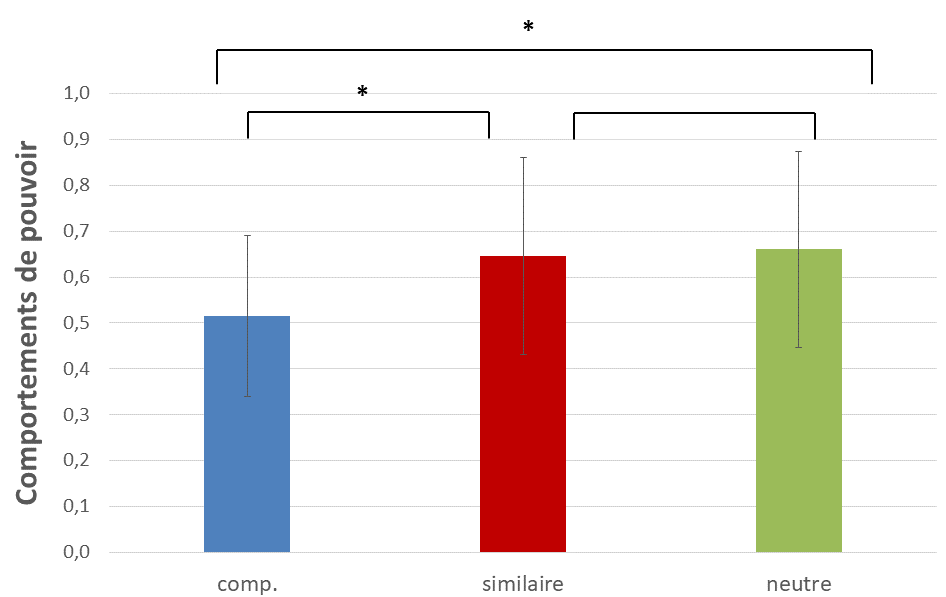
\includegraphics[clip=false]{Figures/chap7/pow.png}
		}
		
		\subfloat[Perception de l'agent des comportements de dominance exprimés par les participants]{
			\begin{tabular}{ l c c c c c }
				\hline
				\textbf{ }& \textbf{Agent Comp.} & &  \textbf{Agent similaire} & & \textbf{Agent neutre} \\ 
				\hline
				\newline Moy. & 0.51 && 0.64 && 0.66 \\
				\newline SD & 0.17 && 0.21 && 0.219   \\
				\hline
				
			\end{tabular}
		}
		\caption{Résultats pour la variation des comportements de dominance à travers les interactions.}
		\label{fig:dom}
	\end{figure}
	
	\section{Discussion}
	\label{sec:discussion}
	En général, toutes nos hypothèses ont été validées. Ces résultats appuient la validité de notre modèle négociation collaborative et de théorie de l'esprit dans le cadre d'une interaction agent/humain.   
	
	\subsection{Perception des comportements des agents}
	Notre hypothèse H1 (\textit{les comportements de complémentarité et de similarité des agents virtuels sont perçus par les participants}) est partiellement validée. 
	
	Quatre comportements de dominance ont été pris en compte pour mesurer la stratégie de négociation. 
	Les participants ont été en mesure de distinguer une différence significative de trois comportements sur quatre entre leurs stratégie et celle de l'agent complémentaire.
	
	En effet, les participants ont perçu une différence entre leurs niveau d'exigence et de concessions \textbf{D3}, \textbf{D2}, ainsi que la prise en compte des préférences de l'autre\textbf{D1}. Cependant, aucune différence n'a été perçu concernant les comportements de leadership durant la négociation \textbf{D4}. 
	
	Concernant, les comportements de l'agent neutre, ce dernier a été perçu comme significativement complémentaires aux utilisateurs pour les comportements \textbf{D1}, \textbf{D2} et \textbf{D3}. 
	Toutefois, comme l'agent complémentaire, aucune différence n'a été perçue dans les comportements relatifs à \textbf{D4} entre l'agent neutre et les participants. 
	
	Nous avons étudié les données afin de comprendre pourquoi les participants ne percevaient pas de différence dans les comportements de leadership. 
	
	Concernant l'agent complémentaire, les comportements de leaderships ont pu être masqué à cause de  sa stratégie d'adaptation qui modifié ses comportements de dominance à chaque tour de parole.
	
	En outre, l'aspect collaboratif de la négociation pourrait avoir atténué la perception du leadership dans la négociation ce qui pourrait expliquer le cas de l'agent neutre. 
	
	Enfin, l'absence de résultats pour les deux agents nous amènent à nous questionner sur les items proposés pour mesurer le leadership. 
	Il serait intéressant de faire une évaluation post-hoc afin de demander aux participants le types de comportements qu'identifieraient le leadership durant la négociation.
	
	En parallèle, les participants ont perçu une similarité entre leurs comportements et ceux de l'agent similaire. En moyenne, pour chaque comportement, les valeurs assignés en auto-attribution et en hétéro sont très proches. De plus, l'absence de différence significative appuie ce résultat. Nous sommes conscients que l'absence de différence n'est pas une assurance de similarité de perception. Cependant, il est difficile de trouver un calcul statistique qui assure la similarité entre deux populations.
	
	D’un point de vue plus général, les résultats obtenus appuient la cohérence de notre modèle de décision tant sur la perception des comportements de dominance que sur la capacité de l'agent à percevoir les comportements de son interlocuteur et de s'y adapter correctement.  
	
	Par ailleurs, la perception des comportements de l'agent neutre comme complémentaires à ceux des participants soutient que la relation interpersonnelle de dominance qui s'établie au cours de l'interaction est complémentaire \cite{burgoonnonverbal}. En effet, indépendamment des deux autres agents où nous avions manipulé l'adaptation de l'agent, dans la condition neutre l'agent ne s'adapte pas aux comportements du participant. Néanmoins, les résultats démontrent que le participant s'est adapté aux comportements exhibés par l'agent et a ainsi établie une relation interpersonnelle de dominance complémentaire.
	
	\subsection{Gain commun}
	Notre seconde hypothèse (\textit{Les négociateurs atteignent un gain commun plus important quand les négociateurs établissent une relation de dominance complémentaire.}) est validée. 
	
	Nous avons en premier temps demandé aux participants de relater leur avis sur le restaurant choisi pour chaque négociation.
	En général, les participants ont été satisfaits du choix final et le trouvaient équitable pour toutes les négociation. 
	En analysant le valeur de satisfiabilité du restaurant choisi pour les préférences des participants (voir table \ref{tab:gainPerceptif}), les valeurs étaient autour de 0.7 (\emph{min =0.69, max = 0.73}). 
	
	Cependant, en analysant la valeur de satisfiabilité pour les préférences de l'agent,  en moyenne, seul l'agent complémentaire a pu converger vers un restaurant qui respecte ses préférences (\emph{M = 0.53, SD = 0.2}). 
	
	
	\begin{table}
		\centering
		\caption{Moyenne des valeurs de satisfiabilité du restaurant choisi pour chaque négociateur} 
		\begin{tabular} {lcccccccc}
			\hline
			& \multicolumn{2}{c}{Agent Comp.} & & \multicolumn{2}{c}{Agent similaire}& & \multicolumn{2}{c}{Agent neutre} \\ % column 4 blank, for spacing
			\cline{2-3} \cline{5-6} \cline{8-9} % horizontal lines connecting cols. 2-3, 5-6
			& Participant & Agent & & Participant & Agent & &  Participant & Agent \\ \hline
			Moy. &0,71 & 0,53 & &  0,69 & 0,33 & & 0,73 & 0,34 \\
			SD & 0,2 & 0,24 & &  0,18 & 0,19 & & 0,18 & 0,16 \\
			\hline
		\end{tabular}
		\label{tab:gainPerceptif}
		
	\end{table}
	
	Concernant l'agent similaire, la moyenne de satisfiabilité est assez basse. Ceci est causé par le fait que les négociateurs ne communiquaient pas bien durant la négociation. Par conséquent, la négociation durait plus longtemps causant la chute de la courbe de concession $Self$. De ce fait, l'agent faisait plus de concession et finissait par accepter un restaurant dont la satisfiabilité n'était pas élevé (\emph{M = 0.33, SD = 0.18}).
	
	Concernant l'agent neutre qui n'est pas très dominant, il est normal que dans la majorité des cas, la courbe de concession finissait par décroitre menant l'agent à faire des concessions importantes. Ceci explique la moyenne de satisfiabilité atteinte par l'agent neutre  (\emph{M = 0.34, SD = 0.16}).
	
	Cette analyse confirme les résultats de l'étude objective menée.
	Pour toutes les négociations, nous avons comparé le gain commun et nous avons observé qu'il était significativement plus important durant les négociations avec l'agent complémentaire comparé aux autres agents. De plus, les négociateurs avaient de meilleurs gains durant la négociation avec l'agent neutre comparé à l'agent similaire. Ceci prouve que la relation complémentaire qui s'est installé durant la négociation avec l'agent neutre a permet un meilleurs échange d'information. 
	
	Ces résultats confirme que les négociateurs communiquent mieux et par conséquent négocient mieux dans le cadre d'une relation complémentaire de dominance.  
	
	
	\subsection{Tours de paroles}
	Notre hypothèse H3 (\textit{La négociation converge plus rapidement dans le cas où les négociateurs ont un relation de dominance complémentaire. }) est validée. En effet, la négociation convergeait en moyenne plus rapidement quand une relation de dominance complémentaire s'établissait entre l'agent et le participant. De plus, dans cette même condition le gain commun atteint par les négociateurs était plus important. Ainsi, ces résultats appuient les théories de  psychologie sociales selon lesquelles la relation interpersonnelle de dominance améliore la coordination et l'échange d'informations.
	
		
	En ce qui concerne l'agent neutre, la négociation convergeait rapidement à cause de deux raisons. Premièrement, avec une valeur de dominance initialisé à 0.5, l'agent avait un niveau d'exigence moyen ce qui facilitait le processus pour trouver un compromis. 
	Deuxièmement, d'après nos résultats, dans cette condition, une relation complémentaire de dominance s'était établie entre les négociateurs ce qui facilitait la coordination. 
	
	En conclusion, la relation interpersonnelle de dominance améliore la coordination et l'échange d'information qui résulte en des processus de négociation court et plus efficaces. 
	
	\subsection{Appréciation de l'agent}
	Nos hypothèses H4 (\textit{Le négociateur se sent plus à l'aise avec un partenaire qui exprime un comportement complémentaire})  et H5 (\textit{ La complémentarité dans la relation de dominance augmente l'appréciation entre les négociateurs.}) sont validées. 
	
	Pour l’appréciation, les scores sont au dessus de la moyenne pour tous les agents. Ce pourrait être le reflet d’un léger biais positif envers les agents. Toutefois, l'analyse des différence a révélé que les participants ont significativement plus apprécié la négociation avec l'agent complémentaire que l'agent similaire. De même, les participants ont jugé que l'agent neutre était aussi plus agréable que l'agent similaire. 
	
	En outre, nous avons analysé le confort ressenti lors de la négociation. Globalement, les participants se sont senti détendus durant la négociation et ont trouvé la négociation confortable avec tous les agents.  
	
	L'analyse de variance a révélé que les participants se sont plus sentis à l'aise avec l'agent complémentaire qu'avec l'agent similaire. Cependant, aucune différence n'a été perçu entre l'agent complémentaire et l'agent neutre, et entre l'agent neutre et l'agent similaire.
	
	En plus du confort, nous avons analysé la facilité de collaborer avec l'agent durant la négociation. Les résultats montent que les participants ont perçu le processus de négociation comme plus aisé avec l'agent complémentaire et l'agent neutre qu'avec l'agent adoptant une stratégie similaire à la leurs. 
	
	Ces résultats confirment nos hypothèses. Les participants préfèrent négocier avec un partenaire avec lequel ils ont établi une relation complémentaire qu'avec un négociateur qui exhibe des comportements de dominance similaires. 
	
	
	\section{Conclusion}
	Pour cette quatrième étude, nous avions pour objectif d'étudier l'effet de la relation de dominance sur la négociation entre un agent et un participant humain. Nous nous sommes basés sur les travaux de Tienders et Wiltermuth \cite{wiltermuth2009benefits,tiedens2003power} qui affirment que la complémentarité dans la relation de dominance avait un impact positif sur la négociation. 
	
	Nous avons implémenté trois agents négociateurs adoptant trois stratégies différentes, un agent complémentaire, un agent similaire et un agent neutre. 
	63 participants ont pris part à  des négociations collaboratives avec ces agents dans le but de trouver un restaurant qui satisfassent leurs préférences. 
	
	Les résultats ont confirmé la majorité de nos hypothèses et nous ont permis d'aller plus loin dans l'analyse des comportements de dominance dans la négociation. 
	
	D'abord, nous avons pu validé notre modèle de la théorie de l'esprit dans le cadre d'une interaction avec un utilisateur humain. 
	Les résultats montrent que les participants ont été capables de percevoir une différence dans les stratégies qu'adoptaient les agents. Ceci nous permet de valider la robustesse des prédictions de notre notre modèle. 
	
	Par ailleurs, toutes les hypothèses relatives à l'effet positif de la relation de dominance complémentaire ont été validées. Quand les négociateurs établissaient une relation de dominance complémentaire, ils atteignaient un meilleur gain commun et ceux dans un délais plus court comparés aux autres configurations. La négociation était vécue comme plus agréable et confortable et les négociateurs semblaient mieux collaborer. 
	
	Les résultats ont aussi révélés des comportements qui soutiennent les travaux en psychologie sociale. En effet, en analysant les comportements exprimés lors des négociations avec l'agent neutre, nous nous sommes rendu compte qu'une relation complémentaire de dominance s'était installé entre les négociateurs. Ces résultats appuient la définition de Dunbar and Burgoon \cite{dunbar2005perceptions} qui affirment que la relation de dominance est forcément complémentaire. En outre, la relation de dominance étant interpersonnelle, elle s'établie durant l'interaction. Ce point a aussi été validé par nos analyses qui nous ont permis de montrer que les participants ont adopté des comportements de dominance différents d'une négociation à une autre. Cela suggère que les négociateurs s'adapte à leur interlocuteur pour définir une relation de dominance propre à l'interaction. 